\documentclass[11pt]{article}
\usepackage[margin=1in]{geometry}
\usepackage{amsmath,amssymb,mathtools,booktabs,longtable,array,graphicx}
\usepackage[hidelinks]{hyperref}
\usepackage{microtype}
\newcommand{\dd}{\mathrm{d}}
\newcommand{\E}{\mathbb{E}}
\newcommand{\Var}{\operatorname{Var}}
\newcommand{\ind}{\mathbf{1}}
\newcommand{\R}{\mathbb{R}}
\newcommand{\argmax}{\operatorname*{arg\,max}}
\newcommand{\argmin}{\operatorname*{arg\,min}}
\setlength{\parindent}{0pt}
\setlength{\parskip}{5pt}
\setlength{\LTpre}{5pt}
\setlength{\LTpost}{5pt}
% Keep each derivation together; allow page breaks between equations.
\setlength{\jot}{5pt}
\title{Update\\Mason 2YP}
\author{}
\date{November 1, 2026}
\begin{document}
\maketitle
\tableofcontents
\clearpage

\section{Empirical demand}
\subsection{Notation}
\small
\begin{longtable}{p{.27\linewidth}p{.67\linewidth}}
\toprule Symbol & Definition\\\midrule\endhead
$i$ & Household.\\
$t\in\mathcal T_i$ & Retained household purchase week, ending Saturday.\\
$\mathcal H_i$ & Observed purchase weeks used to construct history, including weeks subsequently excluded from the likelihood.\\
$j,k\in\mathcal J$ & Flavor categories; $\mathcal J=\{\mathrm{other},\mathrm{berry},\mathrm{plain}\}$.\\
$0$ & Outside alternative, included in the reported fit.\\
$Q_{ijt}$, $Q_{it}$ & Quantity purchased of flavor $j$; total inside quantity $Q_{it}=\sum_jQ_{ijt}$.\\
$x_{ijt}$ & Inside quantity share of flavor $j$, $Q_{ijt}/Q_{it}$.\\
$S_{ijt}$, $N_{ijt}$ & Cumulative own-flavor share stock and immediately preceding calendar week's other-flavor share.\\
$\lambda$, $\Xi_{ijt}$ & Fixed history weight and combined history index; $\lambda=0.7$.\\
$p_{ijt}$ & Exposure-store flavor price.\\
$v_{ijt}$, $\widehat v_{ijt}$ & First-stage price disturbance and estimated residual.\\
$b_0$ & Common inside intercept relative to the outside alternative.\\
$\beta_j$ & Flavor intercept relative to other; $\beta_{\mathrm{other}}=0$ in the reported fit.\\
$\alpha_i$, $\mu_\alpha$, $\sigma_\alpha$ & Positive price sensitivity and mean/SD of its logarithm. Price enters utility as $-\alpha_i p$.\\
$\gamma_i$, $\mu_\gamma$, $\sigma_\gamma$ & Household history coefficient, common across flavors, and its population mean/SD.\\
$\rho$ & Common coefficient on the price-control residual.\\
$\varepsilon_{ijt}$, $V_{ijt}$, $U_{ijt}$ & Unit-scale type-I extreme-value shock, deterministic utility, and total utility.\\
$P_{ijt}$ & Conditional choice probability for given household type.\\
\bottomrule
\end{longtable}
\normalsize

\subsection{Price equation and control residuals}
Let $m$ index consumer DMAs and $m_{it}$ be household $i$'s DMA in week $t$.
$\mathcal Q_{mt}$ contains the distinct store--week--UPC price quotes in DMA
$m$, pooling all flavors. Their count and price sum are
\begin{equation}
\begin{aligned}
n_{mt}&=|\mathcal Q_{mt}|,
\end{aligned}
\end{equation}
\begin{equation}
\begin{aligned}
P_{mt}&=\sum_{q\in\mathcal Q_{mt}}p_q,
\end{aligned}
\end{equation}
The instrument $z_{it}$ is the same-week mean price outside the household's DMA:
\begin{equation}
\begin{aligned}
z_{it}&=\frac{\sum_{m\ne m_{it}}P_{mt}}{\sum_{m\ne m_{it}}n_{mt}},\qquad \sum_{m\ne m_{it}}n_{mt}>0,
\end{aligned}
\end{equation}
\begin{equation}
\begin{aligned}
p_{ijt}&=\pi_j z_{it}
 +\tau_{jt}+\kappa_{j,m_{it}}+v_{ijt},\qquad (i,t)\in\mathcal D_j.
\end{aligned}
\end{equation}
Here $\pi_j$ is the instrument slope
and $\tau_{jt}$ and $\kappa_{jm}$ are flavor-specific week and DMA fixed effects.
$\mathcal D_j$ contains the usable household--weeks for flavor $j$.
The same $z_{it}$ enters each flavor equation. Each household--week has equal first-stage weight.
The table reports the one-instrument Wald statistic $F_j$.

% First-stage results from res_hess.
\begin{table}[htbp]\centering\small
\caption{Price first stages}
\begin{tabular}{lrrrrrr}\toprule
Flavor & $\widehat\pi_j$ & Cluster SE & $F_j$ & Partial $R^2$ & Observations & Households\\\midrule
Other & -35.1444 & 0.4351 & 6,525.21 & 0.0207 & 1,323,901 & 69,713 \\
Berry & -36.9119 & 0.6256 & 3,481.18 & 0.0219 & 486,475 & 54,666 \\
Plain & -31.5474 & 1.2951 & 593.33 & 0.0087 & 195,107 & 34,495 \\
\bottomrule
\end{tabular}
\end{table}

\subsection{Utility, heterogeneity, and choice probabilities}
\emph{Fatigue} is a decline in utility from a flavor as the household accumulates
past purchases of that flavor. \emph{Novelty} is a utility gain from choosing a
flavor different from those purchased in the immediately preceding calendar
week. Define the corresponding history measures by
\begin{equation}
\begin{aligned}
S_{ijt}&=\sum_{\substack{s\in\mathcal H_i\\s<t}}x_{ijs},
&N_{ijt}&=\begin{cases}
\sum_{k\ne j}x_{ik,t-1},&t-1\in\mathcal H_i,\\
0,&t-1\notin\mathcal H_i,
\end{cases}\\
\Xi_{ijt}&=(1-\lambda)N_{ijt}-\lambda S_{ijt},
&\lambda&=0.7.
\end{aligned}
\end{equation}
Thus $\gamma_i\Xi_{ijt}=0.3\gamma_iN_{ijt}-0.7\gamma_iS_{ijt}$:
positive $\gamma_i$ implies both fatigue and a preference for novelty, while
negative $\gamma_i$ implies reinforcement from accumulated own-flavor purchases
and a preference for repeating recent flavors. Fatigue accumulates without
depreciation; novelty depends only on the preceding calendar week and is zero
after a purchase gap. The fixed weight $\lambda$ ties the two effects together,
so they are not separately estimated.

\begin{equation}
\begin{aligned}
U_{ijt}&=V_{ijt}+\varepsilon_{ijt},
\end{aligned}
\end{equation}
\begin{equation}
\begin{aligned}
V_{ijt}&=b_0+\beta_j-\alpha_i p_{ijt}+\gamma_i\Xi_{ijt}+\rho\widehat v_{ijt},
\end{aligned}
\end{equation}
\begin{equation}
\begin{aligned}
\beta_{\mathrm{other}}&=0,
\end{aligned}
\end{equation}
The household type components $Z_{i\alpha}$ and $Z_{i\gamma}$ are independent
standard normals, fixed over each household's history:
\begin{equation}
\begin{aligned}
\log\alpha_i&=\mu_\alpha+\sigma_\alpha Z_{i\alpha},\qquad \alpha_i>0,
\end{aligned}
\end{equation}
\begin{equation}
\begin{aligned}
\gamma_i&=\mu_\gamma+\sigma_\gamma Z_{i\gamma},
\end{aligned}
\end{equation}
\begin{equation}
\begin{aligned}
\begin{pmatrix}Z_{i\alpha}\\Z_{i\gamma}\end{pmatrix}&\sim N(\boldsymbol0,I_2),
\end{aligned}
\end{equation}
Let $\mathcal A_{it}$ contain the inside flavors with finite positive prices
at the household's exposure store. Conditional on household type,
\begin{equation}
\begin{aligned}
P_{ijt}(\alpha_i,\gamma_i)&=\frac{\exp(V_{ijt})}{1+\sum_{k\in\mathcal A_{it}}\exp(V_{ikt})},\qquad j\in\mathcal A_{it},
\end{aligned}
\end{equation}

\subsection{Unaggregated flavor concentration}
Let $\mathcal F$ be the detailed flavor labels and $Q_{ift}$ the quantity of
flavor $f$ bought by household $i$ in week $t$. Household full-history quantity
shares $w_{if}$ and flavor HHI $H_i$ are
\begin{equation}
\begin{aligned}
w_{if}&=\frac{\sum_{t\in\mathcal H_i}Q_{ift}}{\sum_{g\in\mathcal F}\sum_{t\in\mathcal H_i}Q_{igt}},
\end{aligned}
\end{equation}
\begin{equation}
\begin{aligned}
\sum_{f\in\mathcal F}w_{if}&=1,
\end{aligned}
\end{equation}
\begin{equation}
\begin{aligned}
H_i&=\sum_{f\in\mathcal F}w_{if}^2.
\end{aligned}
\end{equation}
\begin{figure}[htbp]\centering
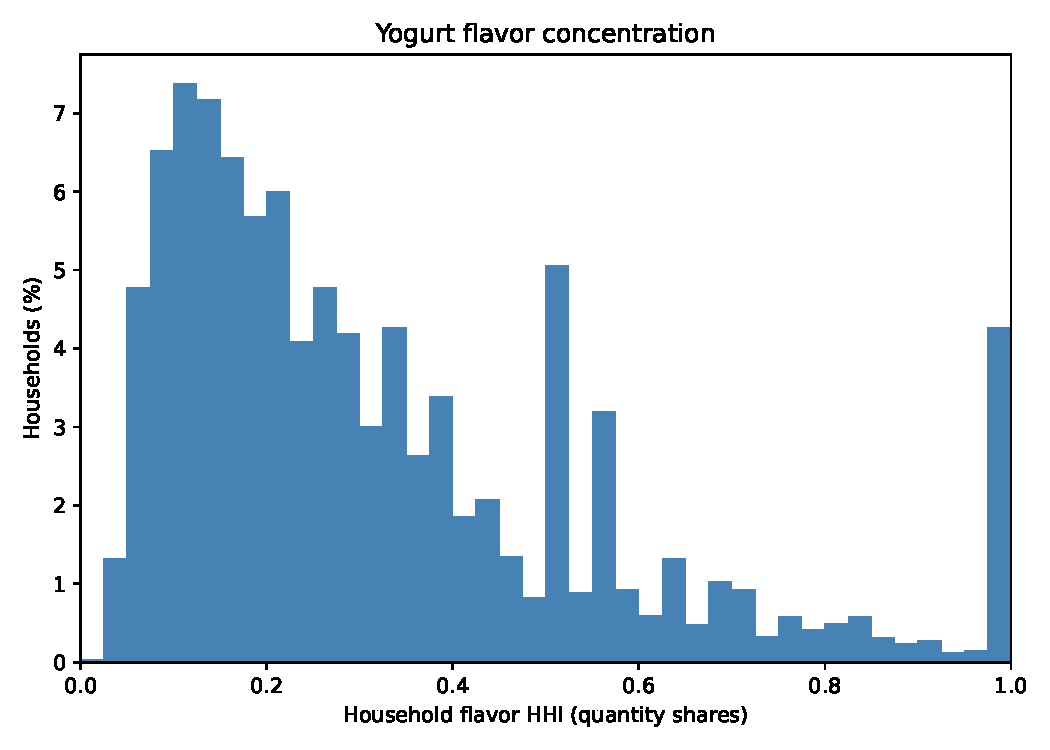
\includegraphics[width=.83\linewidth]{assets/flavor_hhi_histogram.pdf}
\caption{Household flavor HHI; unaggregated flavor labels, package-quantity shares.}
\end{figure}

\begin{figure}[htbp]\centering
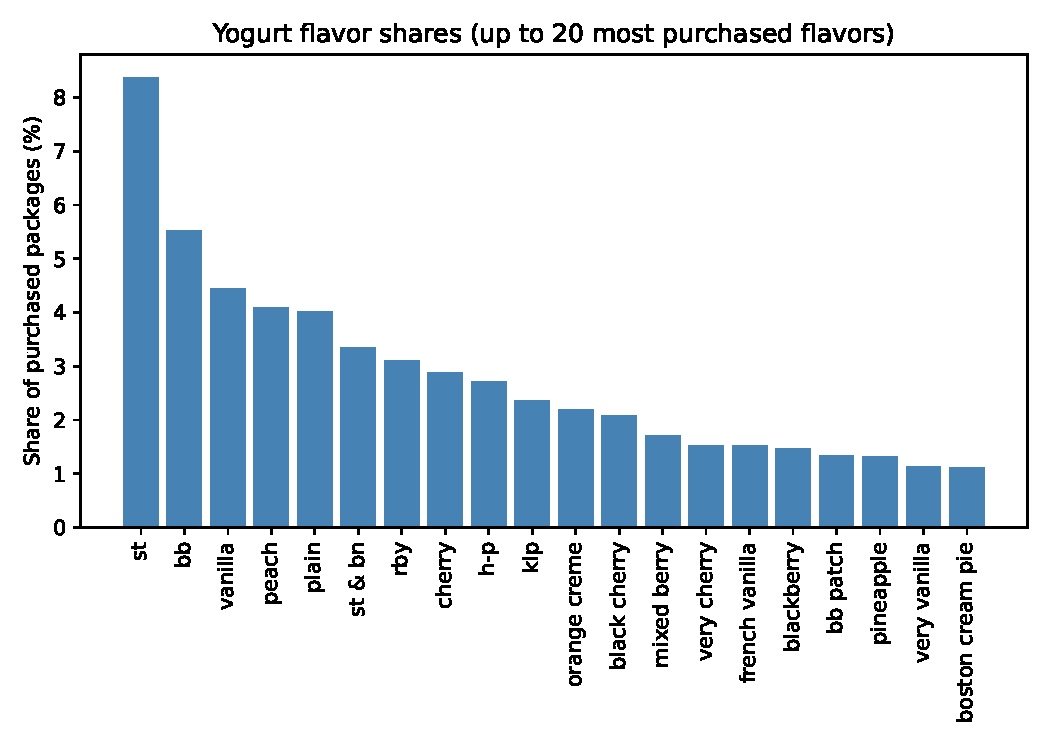
\includegraphics[width=.95\linewidth]{assets/flavor_shares.pdf}
\caption{Package-quantity shares; 20 most purchased unaggregated flavor labels.}
\end{figure}

\clearpage

\subsection{Summary statistics}
The descriptive sample covers 2006--2015. Trips, UPCs, and quantity purchased in the matched yogurt column refer
to yogurt only.

\begin{table}[htbp]\centering\small
\caption{Household purchase summaries}
\label{tab:sample-summary}
\begin{tabular}{lrr}\toprule
Statistic & Full panel & Matched yogurt\\\midrule
Households & 37,827 & 15,106\\
Mean observed panel years & 3.96 & 3.16\\
Mean trips per household & 493.13 & 20.26\\
Mean trips per approximate observed week & 2.27 & 0.11\\
Median trips per approximate observed week & 1.93 & 0.07\\
Mean distinct UPCs per household & 1178.31 & 13.89\\
Mean quantity purchased per household & 4669.07 & 93.77\\
One-person households (\%) & 100.00 & 100.00\\
Two-person households (\%) & 0.00 & 0.00\\
Hispanic origin (\%) & 3.10 & 2.59\\
\bottomrule\end{tabular}
\end{table}

\begin{table}[htbp]\centering\small
\caption{Yogurt purchase dynamics: detailed flavors and estimation categories}
\label{tab:dynamics-summary}
\begin{tabular}{lrr}\toprule
Statistic & Detailed flavors & Three categories\\\midrule
Households & 15,106 & 15,106\\
Observed purchase household--weeks & 282,648 & 282,648\\
Mean flavors/categories bought per household & 10.76 & 1.93\\
Mean household flavor HHI & 0.32 & 0.78\\
Mixed-flavor/category weeks (\%) & 37.88 & 17.45\\
Weeks with quantity purchased above seven (\%) & 21.72 & 21.72\\
Eligible adjacent single-flavor/category week pairs & 30,392 & 48,166\\
Switch rate among eligible pairs (\%) & 46.75 & 12.85\\
Mean single-flavor/category spell length (weeks) & 1.10 & 1.22\\
Median gap between purchase weeks (weeks) & 3.00 & 3.00\\
\bottomrule\end{tabular}
\end{table}
An eligible transition requires purchases in consecutive calendar weeks and
exactly one flavor (or category) in each week. Mixed baskets and gaps are
excluded from the switch-rate denominator, thus it is illustrative only. Spells count consecutive calendar
weeks with the same single flavor or category; a gap breaks the spell.
HHI uses each household's full-history shares of quantity purchased.

\begin{table}[htbp]\centering\small
\caption{Quantity shares and transitions for the three estimation categories}
\label{tab:category-summary}
\begin{tabular}{lrrrr}\toprule
 & Quantity share (\%) & \multicolumn{3}{c}{Next category (row probabilities, \%)}\\
Category & & Other & Berry & Plain\\\midrule
Other & 78.37 & 92.25 & 5.79 & 1.96\\
Berry & 14.60 & 45.27 & 52.93 & 1.79\\
Plain & 7.03 & 18.09 & 1.85 & 80.06\\
\bottomrule\end{tabular}
\end{table}
\clearpage

\subsection{Results}
\begin{table}[htbp]\centering
\caption{Estimation sample and settings; single-person households}
\begin{tabular}{lr}\toprule Setting & Value\\\midrule
Years & 2006--2015 \\
Households & 15,105 \\
Household--weeks & 281,695 \\
Capacity setting & 7 \\
$\lambda$ & 0.7 \\
Integration draws & 32 \\
Optimization starts & 1 \\
Household size & 1 \\
Converged & Yes \\
Parameters at bounds & 0 \\
Negative log likelihood & 1,642,195.0310 \\
\bottomrule
\end{tabular}
\end{table}
\begin{table}[htbp]\centering
\caption{Demand estimates}
\begin{tabular}{lrrc}\toprule Parameter & Estimate & Standard error & 95\% normal interval\\\midrule
$\beta_{\mathrm{berry}}$ & -0.8408 & 0.0349 & [-0.8649, -0.7520] \\
$\beta_{\mathrm{plain}}$ & -0.2454 & 0.0435 & [-0.3069, -0.1461] \\
$\mu_\alpha$ & -0.6585 & 0.1593 & [-0.9152, -0.3818] \\
$\mu_\gamma$ & 0.0405 & 0.0522 & [-0.0818, 0.0531] \\
$\sigma_\alpha$ & 0.8476 & 0.2026 & [0.8051, 1.3620] \\
$\sigma_\gamma$ & 0.0880 & 0.0061 & [0.0815, 0.1007] \\
$\rho$ & 0.2578 & 0.0333 & [0.1858, 0.3275] \\
\bottomrule
\end{tabular}
\end{table}
\begin{table}[htbp]\centering\small
\caption{Implied willingness to pay}
\label{tab:implied-wtp}
\begin{tabular}{lrr}\toprule
Utility coefficient & Mean WTP & Population SD\\\midrule
Inside constant $b_0$ & 2.4170 & 1.8040 \\
Berry vs. other: $\beta_{\mathrm{berry}}$ & -1.1656 & 0.8700 \\
Plain vs. other: $\beta_{\mathrm{plain}}$ & -0.1864 & 0.1391 \\
History index: $\gamma_i$ & -0.1054 & 0.1622 \\
Novelty: $(1-\lambda)\gamma_i$ & -0.0316 & 0.0487 \\
Own-flavor stock: $-\lambda\gamma_i$ & 0.0738 & 0.1135 \\
\bottomrule
\end{tabular}

\begin{minipage}{.95\linewidth}\footnotesize
WTP is in the same monetary units as price, per unit of the indicated regressor.
Flavor coefficients are relative to other; $b_0$ is other versus the outside
option at zero history and control residual. The last two rows hold the other
history regressor fixed, with $\lambda=0.7$.
\end{minipage}
\end{table}
\begin{figure}[htbp]\centering
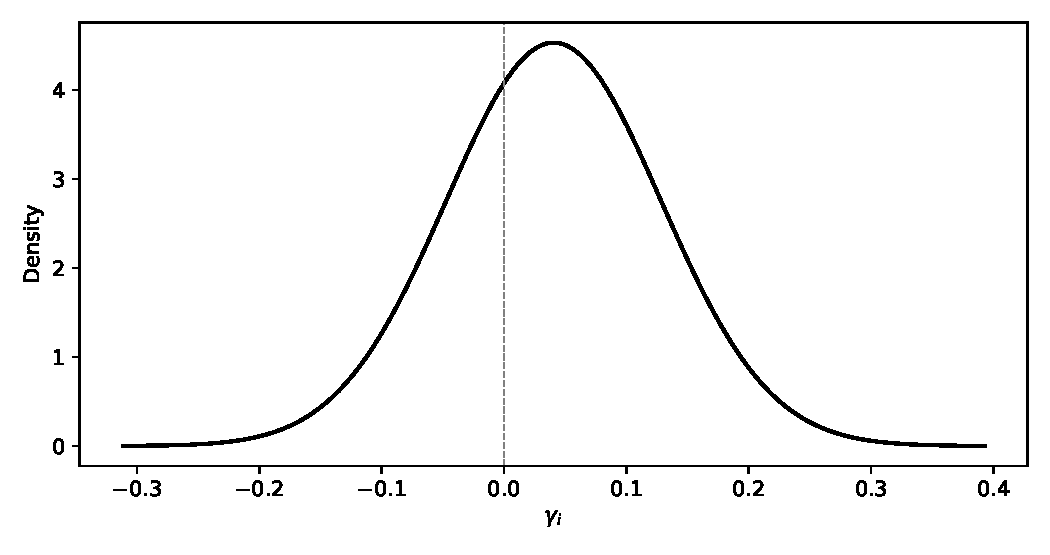
\includegraphics[width=.83\linewidth]{assets/gamma_distribution.pdf}
\caption{Fitted household history coefficient:
$\gamma_i\sim N(-0.0588034,\,0.0634273^2)$.}
\end{figure}


% Saved all-household results retained for reference.
% 
% \begin{table}[htbp]\centering
% \caption{Estimation sample and settings}
% \begin{tabular}{lr}\toprule Setting & Value\\\midrule
% Years & 2006--2015 \\
Households & 15,105 \\
Household--weeks & 281,695 \\
Capacity setting & 7 \\
$\lambda$ & 0.7 \\
Integration draws & 32 \\
Optimization starts & 1 \\
Household size & 1 \\
Converged & Yes \\
Parameters at bounds & 0 \\
Negative log likelihood & 1,642,195.0310 \\
\bottomrule
\end{tabular}
% \end{table}
% \begin{table}[htbp]\centering
% \caption{Demand estimates; household bootstrap}
% \begin{tabular}{lrrc}\toprule Parameter & Estimate & Standard error & 95\% percentile interval\\\midrule
% $\beta_{\mathrm{berry}}$ & -0.8408 & 0.0349 & [-0.8649, -0.7520] \\
$\beta_{\mathrm{plain}}$ & -0.2454 & 0.0435 & [-0.3069, -0.1461] \\
$\mu_\alpha$ & -0.6585 & 0.1593 & [-0.9152, -0.3818] \\
$\mu_\gamma$ & 0.0405 & 0.0522 & [-0.0818, 0.0531] \\
$\sigma_\alpha$ & 0.8476 & 0.2026 & [0.8051, 1.3620] \\
$\sigma_\gamma$ & 0.0880 & 0.0061 & [0.0815, 0.1007] \\
$\rho$ & 0.2578 & 0.0333 & [0.1858, 0.3275] \\
\bottomrule
\end{tabular}
% \end{table}
% \begin{figure}[htbp]\centering
% 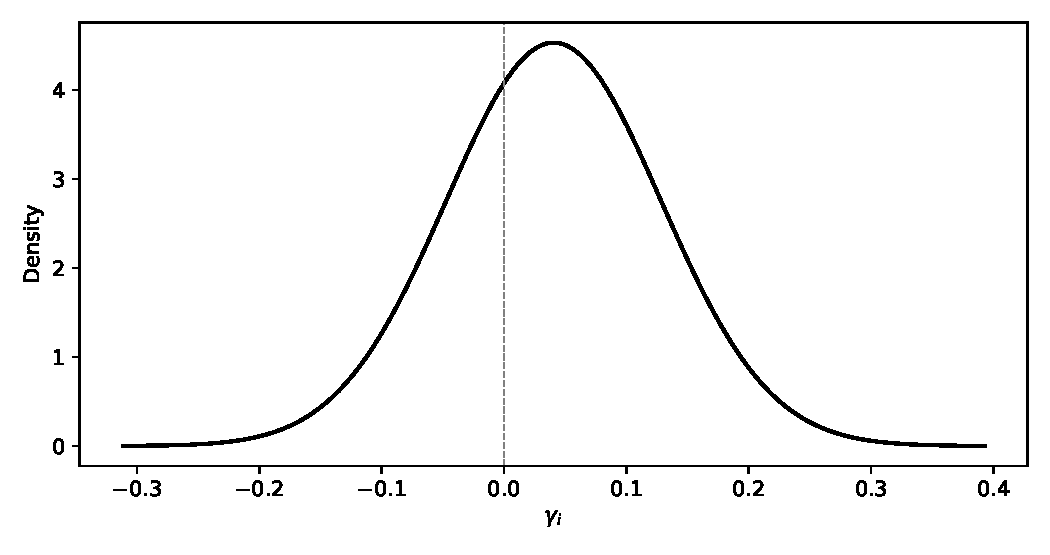
\includegraphics[width=.83\linewidth]{assets/gamma_distribution.pdf}
% \caption{$\gamma_i\sim N(\widehat\mu_\gamma,\widehat\sigma_\gamma^2)$, with $\widehat\mu_\gamma=0.0405473$ and $\widehat\sigma_\gamma=0.0880120$.}
% \end{figure}
% \clearpage
% 
\clearpage

\subsection{Discussion of Results}

I have 15,105 single-person households in my estimation sample, a 30x increase over the past runs. The descriptive yogurt sample has 15,106 households, compared with 15,105 retained for estimation after the usable-week restrictions. In the descriptive yogurt sample, households are observed for an average of about three years and make 20 yogurt-only trips, on average. The full panel covers 37,827 households and averages 493 trips across all products, so that is a different household set. In an approximate observed week, there are only about 0.1 yogurt trips. Households in the descriptive yogurt sample buy about 14 distinct yogurt UPCs as well as about 94 total units of yogurt. Switching stats show that there are nearly 11 flavors bought in the disaggregated sample and about two in the three-flavor category aggregation. Mean within-household flavor HHI in the disaggregated is 0.32 versus 0.78 in the aggregated, expected given how large the categories can be. Similarly, we have more than a third of weeks with a mixed basket in the disaggregated sample versus about 17\% in the three category specification. Switching rate is higher with more flavors to switch between, again to be expected. I think using the disaggregated sample for illustration then three category to ease estimation makes sense. Appreciate thoughts here.

Looking at the within household flavor concentration plot shows that most consumers consume many flavors of yogurt. We do see a large grouping at the single flavor point, but they still only account for about 3\% of households. Interestingly, there is another large cluster around the 50\% point, which is good evidence of switching behavior varying across households. Strawberry yogurt is the most purchased flavor at about 8.5\% of all sales. Notably, nine berry flavors populate the top 20 flavors, showing that it is a good grouping. I do think aggregating "other" into "other fruits", "dessert flavors", and "other" may be good once the three category specification is working as we want it to.

Estimation has taken a massive improvement with the changes to the novelty versus fatigue mechanism in $\Xi$ alongside Josh's proposed changes to changing $\beta_{ij}\rightarrow\beta_j$ and $\gamma_{ij}\rightarrow\gamma_i$. $\gamma$ is now identified with precision, though the effect and spread are quite small. Price sensitivity has a large spread and large negative effect. Looking at the distribution, assumed to be normal, we do see some agents prefer novelty and show fatigue, while most show reinforcement from same-flavor accumulation and prefer repetition in consumption of their preferred products. From the implied willingness to pay, relative to other flavors, berry and plain yogurt would require subsidization for consumers to value the flavors equivalently. For history, we can disaggregate $\gamma$ into the novelty and fatigue terms. Novelty leads to a loss of value of \$-0.03 on average, implying an additional unit (addition to flavor share) reduces the value of a unit. For persistence, about \$0.07 in WTP is added per-unit on average for same flavor accumulation. Both effects hold the other fixed. Overall, this has been a large improvement. I think a lot is due to the sample size growth and then the estimation procedure changes proposed by Josh.

\section{Supply: two-period pricing}
\subsection{Notation}
\small
\begin{longtable}{p{.28\linewidth}p{.66\linewidth}}
\toprule Symbol & Definition\\\midrule\endhead
$t\in\{1,2\}$, $j$, $0$ & Period, inside product, and outside alternative.\\
$x_0=h$, $x_1=a$ & Initial realized choice and realized first-period choice; each belongs to $\{j,0\}$.\\
$\beta$, $\alpha>0$, $\gamma$ & Fixed, firm-observed type's inside intercept, positive price sensitivity, and symmetric switching coefficient. Type indices are suppressed.\\
$c$, $\delta\in(0,1)$ & Marginal cost and discount factor.\\
$p_t(h)$ & Price conditional on preceding realized choice $h$. Prices belong to $\R$.\\
$q(h)$ & Signed history indicator: $q(j)=-1$, $q(0)=1$.\\
$s_t(h)$, $s_{0t}(h)$ & Inside and outside choice probabilities.\\
$W_2(a)$ & Optimized terminal profit conditional on $x_1=a$.\\
$\Pi(p_1;h)$, $\Pi^*(h)$ & Expected discounted profit at candidate first-period price and at its optimum.\\
\bottomrule
\end{longtable}
\normalsize

\subsection{Utilities and shares}
$V_{jt}^{\mathrm{raw}}$ and $V_{0t}^{\mathrm{raw}}$ are deterministic utilities
before subtracting the outside utility. Their difference is $v_t(h)$:
\begin{equation}
\begin{aligned}
V_{jt}^{\mathrm{raw}}&=\beta-\alpha p_t+\gamma\ind\{x_{t-1}=0\},
\end{aligned}
\end{equation}
\begin{equation}
\begin{aligned}
V_{0t}^{\mathrm{raw}}&=\gamma\ind\{x_{t-1}=j\},
\end{aligned}
\end{equation}
\begin{equation}
\begin{aligned}
v_t(h)&=V_{jt}^{\mathrm{raw}}-V_{0t}^{\mathrm{raw}}\\[3pt]
&=\beta-\alpha p_t(h)+\gamma[\ind\{h=0\}-\ind\{h=j\}]\\[3pt]
&=\beta-\alpha p_t(h)+q(h)\gamma,
\end{aligned}
\end{equation}
\begin{equation}
\begin{aligned}
s_t(h)&=\frac{e^{v_t(h)}}{1+e^{v_t(h)}},\qquad s_{0t}(h)=1-s_t(h).
\end{aligned}
\end{equation}
\begin{equation}
\begin{aligned}
\frac{\partial s_t}{\partial p_t}&=-\alpha s_t(1-s_t),
\end{aligned}
\end{equation}
\begin{equation}
\begin{aligned}
\left.\frac{\partial s_t}{\partial\gamma}\right|_{p_t,h}&=q(h)s_t(1-s_t),
\end{aligned}
\end{equation}

\subsection{Terminal-period optimization}
A star marks an optimized price or its associated choice probability.
For each $a\in\{j,0\}$:
\begin{equation}
\begin{aligned}
W_2(a)&=\max_{p_2(a)\in\R}s_2(a)[p_2(a)-c],
\end{aligned}
\end{equation}
\begin{equation}
\begin{aligned}
0&=\frac{\partial}{\partial p_2}\{s_2(p_2-c)\}\\[3pt]
&=s_2+(p_2-c)\frac{\partial s_2}{\partial p_2}\\[3pt]
&=s_2-\alpha s_2(1-s_2)(p_2-c),
\end{aligned}
\end{equation}
\begin{equation}
\begin{aligned}
1&=\alpha(1-s_2^*)(p_2^*-c),
\end{aligned}
\end{equation}
\begin{equation}
\begin{aligned}
p_2^*(a)&=c+\frac1{\alpha[1-s_2^*(a)]},
\end{aligned}
\end{equation}
\begin{equation}
\begin{aligned}
W_2(a)&=\frac{s_2^*(a)}{\alpha[1-s_2^*(a)]}.
\end{aligned}
\end{equation}

\subsection{First-period optimization}
\begin{equation}
\begin{aligned}
\Pi(p_1;h)&=s_1(h)(p_1-c)+\delta\{s_1(h)W_2(j)+[1-s_1(h)]W_2(0)\}\\[3pt]
&=\delta W_2(0)+s_1(h)[p_1-c+\delta[W_2(j)-W_2(0)]],
\end{aligned}
\end{equation}
\begin{equation}
\begin{aligned}
\partial_{p_1}\Pi&=s_1+\partial_{p_1}s_1[p_1-c+\delta[W_2(j)-W_2(0)]]\\[3pt]
&=s_1-\alpha s_1(1-s_1)[p_1-c+\delta[W_2(j)-W_2(0)]],
\end{aligned}
\end{equation}
\begin{equation}
\begin{aligned}
0&=1-\alpha(1-s_1^*)[p_1^*-c+\delta[W_2(j)-W_2(0)]],
\end{aligned}
\end{equation}
\begin{equation}
\begin{aligned}
p_1^*(h)&=c+\frac1{\alpha[1-s_1^*(h)]}-\delta[W_2(j)-W_2(0)],
\end{aligned}
\end{equation}
\begin{equation}
\begin{aligned}
\Pi^*(h)&=\delta W_2(0)+\frac{s_1^*(h)}{\alpha[1-s_1^*(h)]}.
\end{aligned}
\end{equation}

\subsection{Profit derivative}
\begin{equation}
\begin{aligned}
\frac{\dd\Pi^*(h)}{\dd\gamma}
&=\left.\partial_\gamma\Pi(p_1;h)\right|_{p_1=p_1^*(h)}\\[3pt]
&=\frac{q(h)s_1^*(h)-\delta s_1^*(h)s_2^*(j)
 +\delta[1-s_1^*(h)]s_2^*(0)}{\alpha}.
\end{aligned}
\end{equation}

\subsection{Conditional derivative signs}
\begin{equation}
\begin{aligned}
\frac{\dd\Pi^*(0)}{\dd\gamma}
&=\frac{s_1^*(0)[1-\delta s_2^*(j)]+\delta[1-s_1^*(0)]s_2^*(0)}{\alpha}>0,
\end{aligned}
\end{equation}
\begin{equation}
\begin{aligned}
\frac{\dd\Pi^*(j)}{\dd\gamma}>0
&\iff\delta[1-s_1^*(j)]s_2^*(0)>s_1^*(j)[1+\delta s_2^*(j)].
\end{aligned}
\end{equation}

\subsection{Price ratios and conditional profit for all histories}
For each history $(h,a)=(x_0,x_1)\in\{(0,0),(0,j),(j,j),(j,0)\}$,
\begin{equation}
R_{h,a}=\frac{p_1^*(h)}{p_2^*(a)}.
\end{equation}
Each ratio requires a nonzero denominator. A ratio below one means the
second-period price exceeds the first-period price; a ratio above one means
the first-period price exceeds the second-period price.

Conditional on the realized first-period choice $a$, profit is
\begin{equation}
\Pi^*(h,a)=\ind\{a=j\}[p_1^*(h)-c]+\delta W_2(a).
\end{equation}
The first-period margin is realized, while terminal profit remains expected.
Fully realized two-period profit would also condition on $x_2$. Averaging over
first-period choices recovers optimal expected profit:
\begin{equation}
\Pi^*(h)=s_1^*(h)\Pi^*(h,j)+[1-s_1^*(h)]\Pi^*(h,0).
\end{equation}

\subsection{Numerical specification}
\[
\beta=2,\qquad\alpha=1,\qquad\delta=0.92,\qquad c=0,
\qquad\gamma\in[-3,3]\quad(601\text{ grid points per initial state}).
\]
\begin{table}[htbp]\centering\small
\caption{Selected supply solutions}
\begin{tabular}{crrrrrr}\toprule
$h$ & $\gamma$ & $p_1^*(h)$ & $p_2^*(j)$ & $p_2^*(0)$ & $\Pi^*(h)$ & $\dd\Pi^*(h)/\dd\gamma$\\\midrule
$j$ & -3 & 3.395 & 3.926 & 1.120 & 5.087 & -1.387 \\
$j$ & -1 & 2.236 & 2.557 & 1.567 & 2.669 & -0.959 \\
$j$ & 0 & 2.000 & 2.000 & 2.000 & 1.920 & -0.500 \\
$j$ & 1 & 2.209 & 1.567 & 2.557 & 1.731 & 0.125 \\
$j$ & 3 & 3.592 & 1.120 & 3.926 & 2.702 & 0.668 \\
$0$ & -3 & -0.780 & 3.926 & 1.120 & 0.913 & 0.195 \\
$0$ & -1 & 1.045 & 2.557 & 1.567 & 1.478 & 0.385 \\
$0$ & 0 & 2.000 & 2.000 & 2.000 & 1.920 & 0.500 \\
$0$ & 1 & 2.956 & 1.567 & 2.557 & 2.478 & 0.615 \\
$0$ & 3 & 4.801 & 1.120 & 3.926 & 3.912 & 0.804 \\
\bottomrule
\end{tabular}
\end{table}
\clearpage
\begin{figure}[p]\centering
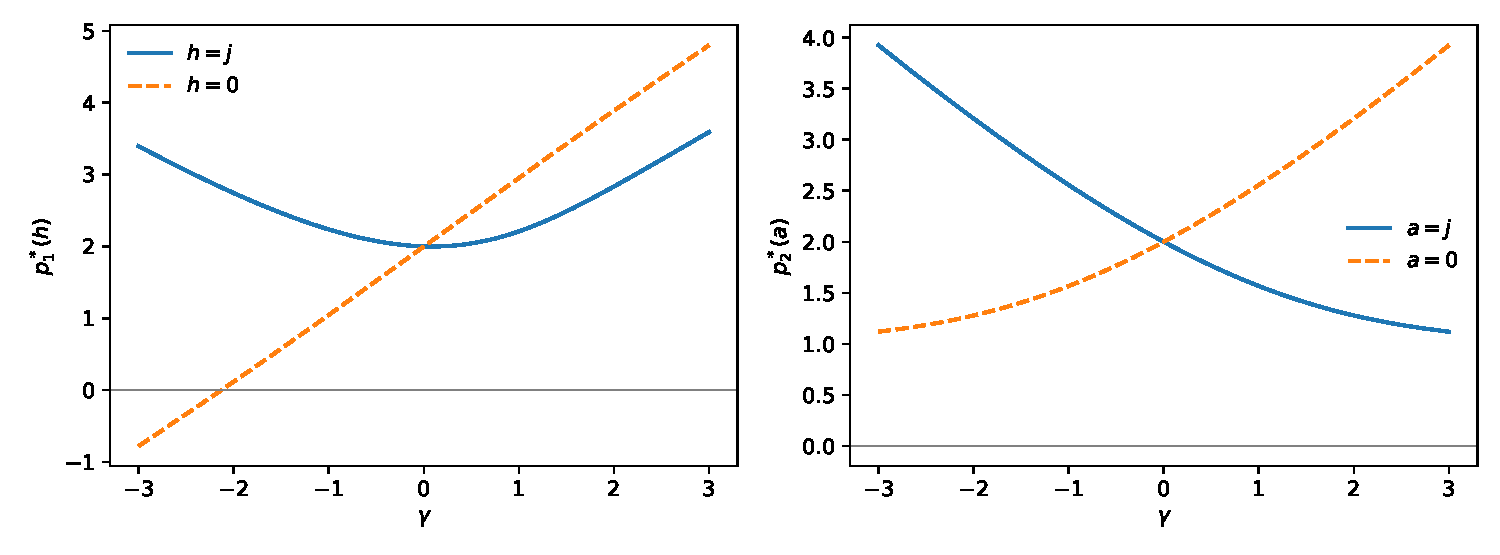
\includegraphics[width=\linewidth]{assets/prices.pdf}
\caption{$p_1^*(h)$ and $p_2^*(a)$; $\beta=2$, $\alpha=1$, $\delta=0.92$, $c=0$.}
\end{figure}
\clearpage
\begin{figure}[p]\centering
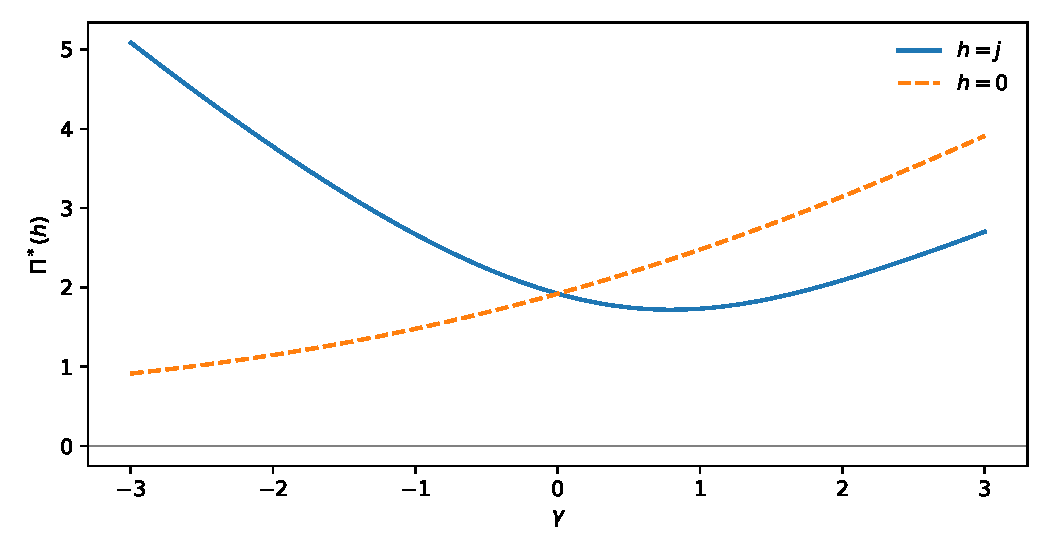
\includegraphics[width=.82\linewidth]{assets/profit.pdf}
\caption{$\Pi^*(h)$; $\beta=2$, $\alpha=1$, $\delta=0.92$, $c=0$.}
\end{figure}
\begin{figure}[p]\centering
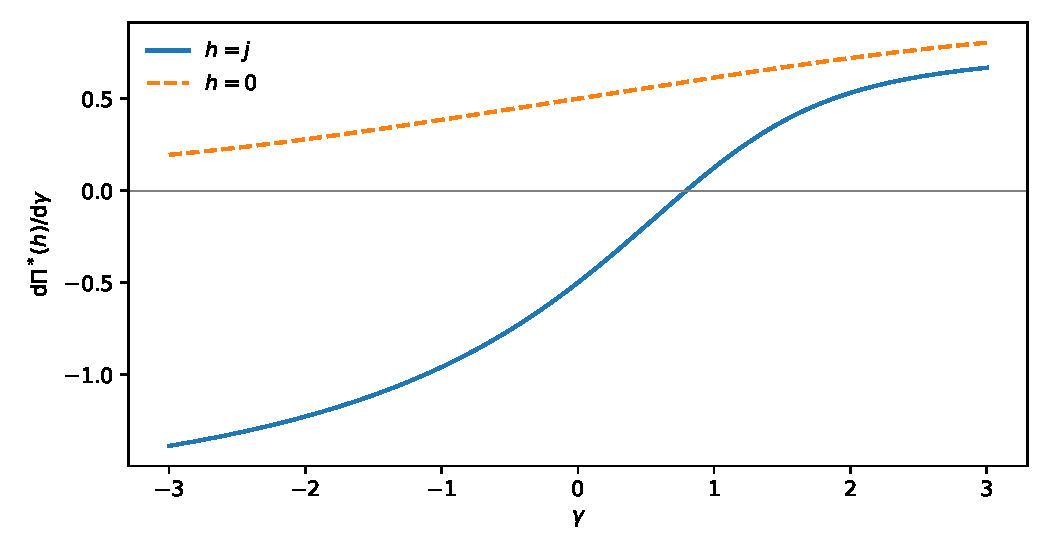
\includegraphics[width=.82\linewidth]{assets/profit_derivative.pdf}
\caption{$\dd\Pi^*(h)/\dd\gamma$; $\beta=2$, $\alpha=1$, $\delta=0.92$, $c=0$.}
\end{figure}
\clearpage
\begin{figure}[p]\centering
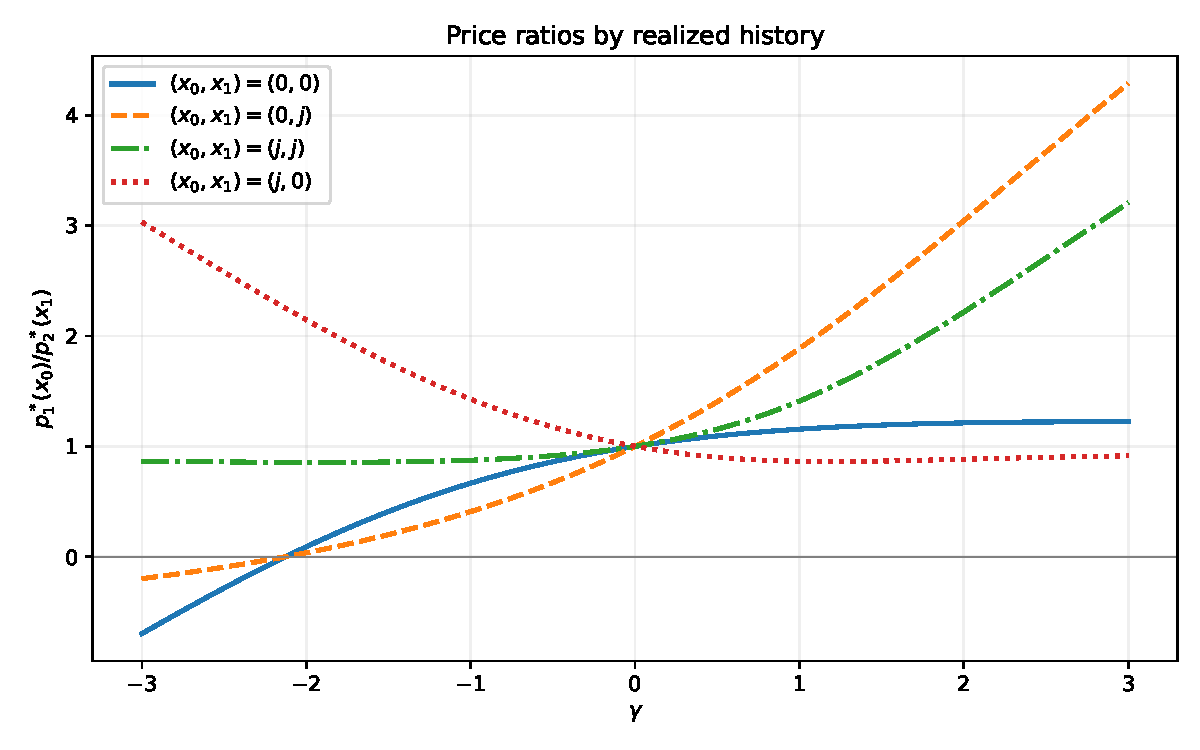
\includegraphics[width=.95\linewidth]{assets/all_state_price_ratios.pdf}
\caption{Price ratios $R_{h,a}=p_1^*(h)/p_2^*(a)$ for all four histories $(h,a)=(x_0,x_1)$; $\beta=2$, $\alpha=1$, $\delta=0.92$, $c=0$.}
\end{figure}
\begin{figure}[p]\centering
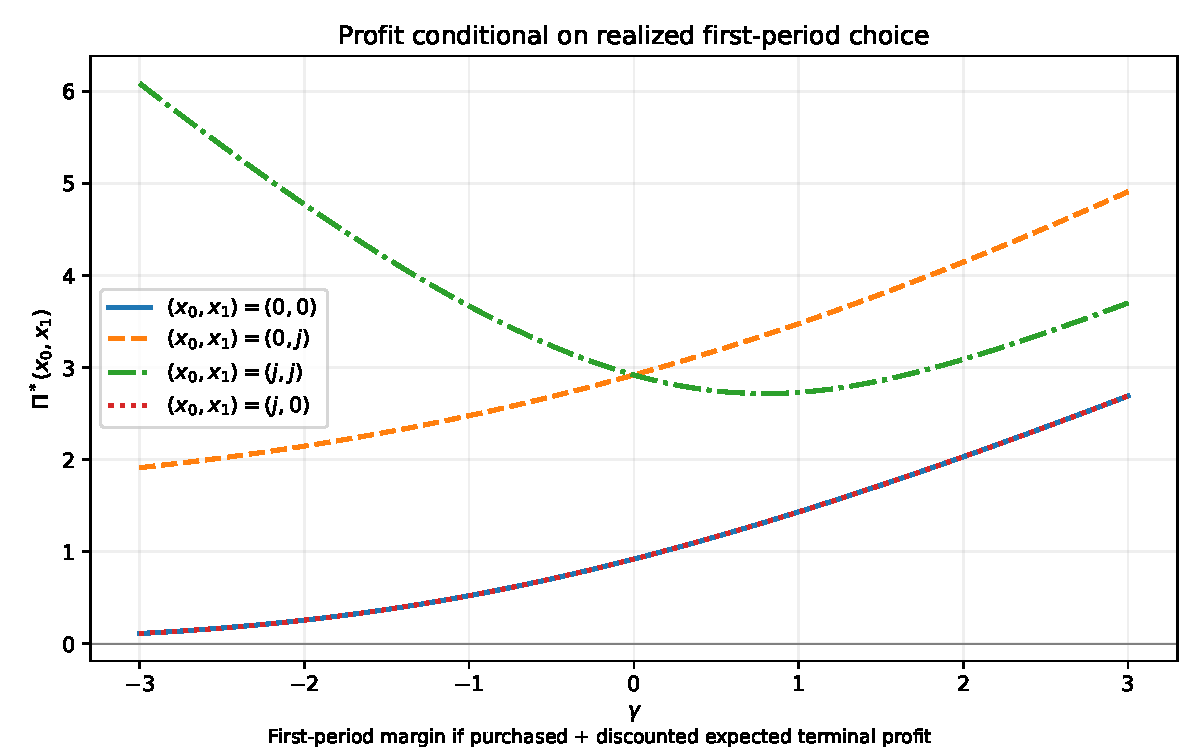
\includegraphics[width=.95\linewidth]{assets/all_state_realized_profit.pdf}
\caption{Conditional profit $\Pi^*(h,a)$ for all four histories. First-period profit is realized and terminal profit is expected. The $(0,0)$ and $(j,0)$ curves coincide; $\beta=2$, $\alpha=1$, $\delta=0.92$, $c=0$.}
\end{figure}
\clearpage
\subsection{Discussion of Supply}

Optimal first-period prices are U-shaped for consumers initially inside
($h=j$), while prices for consumers initially outside ($h=0$) increase with
$\gamma$. Terminal prices depend on the most recent choice: positive $\gamma$
raises willingness to buy after $a=0$ and lowers willingness to buy after
$a=j$.

For negative $\gamma$, persistence supports an induce-then-harvest strategy:
the firm can offer an initially outside consumer a low or even negative
first-period price, then charge a higher terminal price after purchase.
The price ratio $R_{0,j}$ captures this pattern.

For high positive $\gamma$, the timing reverses. Initially outside consumers
want to switch into $j$, allowing the firm to charge a high first-period
price. After purchase, these same consumers want to switch away, so the firm
lowers the terminal price to offset some of the loss of demand. This retention
discount maximizes terminal profit but does not prevent purchase shares from
falling as switching preferences strengthen.

For initially inside consumers, allowing a first-period departure also has
value: choosing $0$ makes the consumer more willing to return in period 2.
When $W_2(0)>W_2(j)$, the first-period pricing condition includes a positive
opportunity cost $\delta[W_2(0)-W_2(j)]$. The firm requires a larger current
margin to compensate for placing a buyer in the less profitable continuation
state. At sufficiently high $\gamma$, first-period prices rise even while the
first-period purchase probability falls.

The conditional-profit curves distinguish margins from the probabilities of
earning them. Both $(0,j)$ and $(j,j)$ receive the same terminal retention
price and continuation value; their profit difference comes entirely from
first-period margins. The rising $(j,j)$ conditional-profit curve at high
$\gamma$ describes a large margin on an increasingly rare first-period
purchase. For $(0,0)$ and $(j,0)$, no first-period margin is earned, so both
conditional profits equal $\delta W_2(0)$. Optimal expected profit weights
each conditional profit by its first-period choice probability.

These simulations use an illustrative calibration. A future step is to
integrate the estimated preference distribution into the pricing exercise
and compare the resulting prices with observed prices.

\end{document}
